% !TeX root = ../../main.tex
\section{Process design data sheets}

\subsection{Key reactor}

\newpage
\subsection{Key Crystalliser}

\newpage
\subsection{Heat exchanger}

\newpage
\subsection{Safety relief valve}

\begin{table}[H]
    \centering
    \begin{tabular}{@{}l|l@{}}
    \toprule
      \textbf{Equipment label}  & PRV-1 on R201\\
       \textbf{Equipment type}  & Safety pressure relief valve \\
       \textbf{Material of construction} & Stainless steel 316 \\
       \bottomrule
    \end{tabular}
\end{table}


\begin{figure}[H]
    \centering
    \begin{subfigure}{0.49\linewidth}
        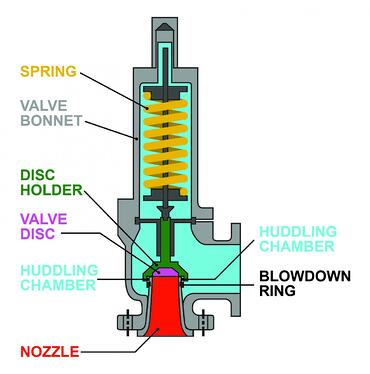
\includegraphics[width=\linewidth]{chapters/Z-support/figures/PSV_Diagram.jpg}
        \caption{AHP}
    \end{subfigure}
    \begin{subfigure}{0.49\linewidth}
        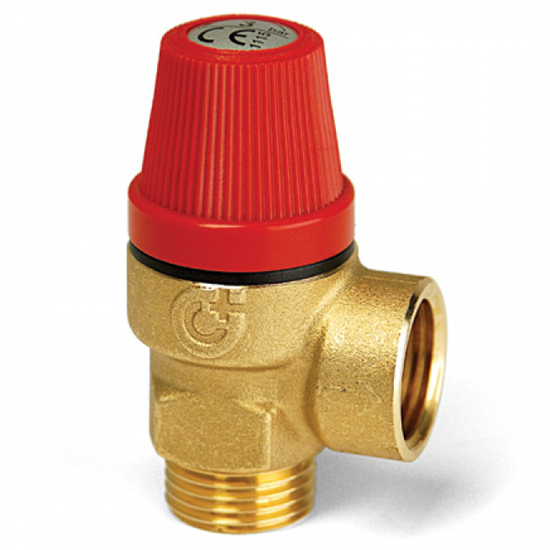
\includegraphics[width=\linewidth]{chapters/Z-support/figures/product_a_l_altecnic-caleffi-safety-relief-valve-1-2-6-bar-312460-small.jpg}
        \caption{TOPSIS}
    \end{subfigure}
    \caption{Sensitivity analysis of AHP and TOPSIS results for nitration catalyst selection.}%
    \label{fig:catalyst}%
\end{figure}

\begin{table}[H]
\centering
\begin{tabular}{@{}l|l|l@{}}
\toprule
\textbf{Specification}                    & \textbf{Value} & \textbf{Units} \\ \midrule
Temperature                               & 60             & °C             \\ \midrule
Max discharge   flowrate                  & 11.779         & kg/hr          \\ \midrule
Ratio of   specific heats (Cp/Cv)  []       & 1.41           &                \\ \midrule
Inlet   pressure, P1                      & 506.625        & kPa            \\ \midrule
Outlet   pressure, P2                     & 101            & kPa            \\ \midrule
Critical   pressure                       & 266.790        & kPa            \\ \midrule
Maximum   allowable accumulated  pressure & 596.544        & kPa            \\ \midrule
Efficient   discharge coefficient  []        & 0.975          &                \\ \midrule
Required   discharge area                 & 11.354         & mm$^2$            \\ \midrule
Nominal nozzle   size                     & 3.80           & mm             \\ \bottomrule
\end{tabular}
\end{table}

\newpage
\subsection{Control valve}

\newpage
\subsection{Pump}

\newpage
\subsection{Storage vessel}

\newpage
\subsection{Flare stack}

\newpage
\subsection{Wash column}

\newpage
\subsection{Air cooler}


